% --- START OF FILE proposal.tex ---

% Ensure 10pt font size is specified
\documentclass[conference, 10pt]{IEEEtran} 

% --- Preamble (Packages, etc.) ---
\usepackage{cite}
\usepackage{amsmath,amssymb,amsfonts}
\usepackage{algorithmic}
\usepackage{graphicx} % Needed for including figures
\usepackage{textcomp}
\usepackage{xcolor}
\usepackage{url} % Needed for \url{} 
\usepackage{float}





\def\BibTeX{{\rm B\kern-.05em{\sc i\kern-.025em b}\kern-.08em
    T\kern-.1667em\lower.7ex\hbox{E}\kern-.125emX}}
    
\begin{document}

% --- Title Block ---
\title{Accelerating Convolution Kernels on Multi-Core CPUs using Parallel Programming}
% --- AUTHORS ---
\author{
    \IEEEauthorblockN{1\textsuperscript{st} Belal Anas Awad}
    \IEEEauthorblockA{\textit{Computer and Systems Eng. Dept.} \\
    \textit{Faculty of Engineering, Ain Shams University}\\
    Cairo, Egypt \\
    21P0072@eng.asu.edu.eg}
\and
    \IEEEauthorblockN{2\textsuperscript{nd} Mohamed Salah Fathy}
    \IEEEauthorblockA{\textit{Computer and Systems Eng. Dept.} \\
    \textit{Faculty of Engineering, Ain Shams University}\\
    Cairo, Egypt \\
    21p0117@eng.asu.edu.eg}
\and
    \IEEEauthorblockN{3\textsuperscript{rd} Salma Mohamed Youssef}
    \IEEEauthorblockA{\textit{Computer and Systems Eng. Dept.} \\
    \textit{Faculty of Engineering, Ain Shams University}\\
    Cairo, Egypt \\
    21P0148@eng.asu.edu.eg}
\and
    \IEEEauthorblockN{4\textsuperscript{th} Salma Hisham Hassan Wagdy}
    \IEEEauthorblockA{\textit{Computer and Systems Eng. Dept.} \\
    \textit{Faculty of Engineering, Ain Shams University}\\
    Cairo, Egypt \\
    21P0124@eng.asu.edu.eg}
}


\maketitle 

% --- Abstract & Keywords ---
\begin{abstract}
Convolution is a fundamental and computationally intensive operation widely used in computer vision and image processing. This project investigates the performance limitations of sequential convolution implementations and explores acceleration using multi-core CPU architectures. We employ profiling techniques to identify bottlenecks, and parallelize the core convolution loops, and conduct a systematic evaluation of the resulting speedup and scalability. The objective is to demonstrate significant performance improvements achievable through standard parallel programming techniques for this common computational kernel, contextualized within the principles of automatic parallelization analysis.
\end{abstract}

\begin{IEEEkeywords}
Parallel Computing, OpenMP, MPI, Image Convolution, Image Processing, Performance Analysis, Multi-core CPU, Kernel Acceleration, Speedup, Scalability
\end{IEEEkeywords}

% ====================================================================
% --- MAIN PROPOSAL CONTENT STARTS HERE ---
% ====================================================================

% --- Introduction ---
\section{Introduction}
Convolution is a foundational operation in image processing and computer vision, 
underpinning tasks such as edge detection, blurring, and feature extraction. It is also a core component in deep learning architectures. 
Despite its importance, convolution is computationally intensive, particularly for high-resolution and multi-channel images, 
due to its repeated access to neighboring pixels and large computational footprint.
Sequential implementations of convolution underutilize modern parallel hardware, leading to inefficient execution and increased processing time. 
Automatic parallelization offers a promising solution by transforming sequential code into parallel code with minimal programmer intervention. 
This process relies on static or dynamic code analysis to identify parallelizable sections,
divide workloads, and coordinate execution across computing resources. 
However, automatic parallelization remains non-trivial due to challenges such as data dependencies, 
load balancing, and communication overhead \cite{hager2021hpc}.
To address these challenges, this project implements and compares three parallelization approaches 
for accelerating sequential 2D convolution kernels using: 
(1) MPI for distributed memory parallelization\cite{toth2016convolution}. 
(2) Combining MPI with OpenMP to leverage both inter-process and intra-process parallelism, improving thread-level concurrency.
MPI enables efficient communication and workload distribution across processes, 
while OpenMP facilitates shared-memory parallelism within nodes \cite{farber2011openmp}. 
(3) Leveraging CUDA for GPU-based acceleration,
capitalizing on massive thread-level parallelism available in modern GPUs \cite{nvidia2021cuda}.
We begin by profiling the sequential code to identify bottlenecks. 
Domain decomposition and thread parallelism techniques will then be applied, tailored to each architecture. 
Each parallelization approach will then be implemented and benchmarked 
to evaluate performance in terms of speedup, scalability, and efficiency.
This work aims to provide insights into the trade-offs and benefits of distributed, shared-memory, and GPU-based parallelization techniques, 
contributing to the broader understanding of high-performance computing in image processing.




% --- PROBLEM DEFINITION ---
\section{Problem Definition}

\subsection{The Convolution Operation}
A convolution operation involves the following detailed steps:

\begin{itemize}
    \item \textbf{Filter Definition:} A small matrix (typically 3×3 or 5×5) is defined as the convolutional kernel.
    \item \textbf{Kernel Traversal:} This kernel moves systematically across the input image from left-to-right and top-to-bottom.
    \item \textbf{Dot Product Computation:} At each location:
    \begin{enumerate}
        \item The kernel is aligned with a portion of the image.
        \item Element-wise multiplication is performed between kernel values and corresponding image pixels.
        \item All products are summed to produce a single output value.
    \end{enumerate}
    \item \textbf{Feature Map Formation:} The results of these computations form a new matrix representing transformed features of the original image.
\end{itemize}

\subsection{Convolution in CNNs}
Convolutional Neural Networks (CNNs) utilize multiple convolutional layers combined with traditional neural network layers. The hierarchical feature extraction process occurs as follows:

\begin{itemize}
    \item \textbf{Layer Progression:}
    \begin{itemize}
        \item Initial layers detect basic features (edges, textures).
        \item Intermediate layers combine these into more complex patterns.
        \item Final layers identify complete components (e.g., facial features, object parts).
    \end{itemize}
    \item \textbf{Implementation Steps:}
    \begin{enumerate}
        \item Kernel alignment at the top-left image pixel.
        \item Precise element-wise multiplication between kernel and image region.
        \item Aggregation of products into a feature map pixel.
        \item Systematic repetition across the entire image with specified stride.
    \end{enumerate}
\end{itemize}

\subsection{Parallelization Approaches}
\subsubsection{Data Parallelism}
Data parallelism is a powerful technique where the same operation (like convolution) is performed on different parts of data simultaneously.

\begin{itemize}
    \item \textbf{Implementation Steps:}
    \begin{enumerate}
        \item \textbf{Partition the input data into smaller chunks (e.g., image tiles):} Each block will be assigned to a thread/process.
        \item \textbf{Apply Convolution in Parallel:} Each thread applies the same kernel on its data block. Since output at each location is independent, there's no data race.
        \item Each unit performs the convolution operation independently on its assigned chunk.
        \item \textbf{Synchronize or Merge Results:} In shared-memory systems (OpenMP, CUDA), threads write to separate output buffers — minimal sync needed. In distributed systems (MPI), use \texttt{MPI\_Gather} or \texttt{MPI\_Reduce} to merge partial outputs.
    \end{enumerate}
    \item \textbf{Advantages:}
    \begin{itemize}
        \item \textbf{Increased Speed:} Each thread or processing unit handles a portion of data, reducing execution time.
        \item \textbf{Scalability:} Works efficiently on multi-core CPUs, GPUs, and clusters (via MPI).
        \item \textbf{Simplicity:} You replicate the same logic across data chunks — easier to manage and debug.
        \item \textbf{Reduced Memory Bottleneck:} Localized data access patterns improve cache utilization and memory access speeds.
        \item \textbf{Portability:} Data parallelism can be implemented with OpenMP (CPU), CUDA (GPU), or MPI (distributed).
    \end{itemize}
\end{itemize}





% --- EVALUATION PLAN ---
\section{Approaches Used}

\subsection{\textbf{CUDA Evaluation and Profiling}}

\textbf{Hardware Platform.} 
The evaluation was performed on a laptop equipped with an \textit{AMD Ryzen\texttrademark~9 5900HS} CPU and a discrete \textbf{NVIDIA GeForce RTX 3050 (6~GB GDDR6)} GPU. This combination supports efficient multi-threaded execution on the host and high-throughput parallel execution on the device. Key hardware specifications:

\begin{itemize}
    \item \textbf{CPU:} 8 cores $\times$ 2 threads/core = 16 logical threads, up to 4.68~GHz
    \item \textbf{Cache:} 512~KB L1, 4~MB L2, 16~MB L3 (shared)
    \item \textbf{Memory:} 16~GB DDR4 @ 3200~MHz, dual-channel
    \item \textbf{GPU:} NVIDIA RTX 3050 Laptop GPU, 2048 CUDA cores, 6~GB GDDR6, boost clock ~1740~MHz
\end{itemize}

\textbf{Software Stack.}
\begin{itemize}
    \item \textbf{OS:} Ubuntu 24.04.2 LTS, Kernel 6.11.0
    \item \textbf{Compiler:} GNU GCC 13.3.0
    \item \textbf{CUDA Toolkit:} 12.9 with Nsight Compute 2025.2.0
    \item \textbf{Profiler:} \texttt{ncu (Nsight Compute)} for GPU kernel-level analysis
\end{itemize}

\textbf{Parallel Convolution using CUDA.}  
The input image is divided into grids of thread blocks. Each thread is assigned to compute a single output pixel by applying a convolution mask to a neighborhood in the input image. To reduce latency from global memory, shared memory is used to cache overlapping image tiles per block. This minimizes redundant memory fetches and increases performance via data reuse.

\textbf{CUDA Execution Model.}  
In CUDA's heterogeneous model, the CPU (host) handles memory allocation and kernel invocation, while the GPU (device) performs actual computation across thousands of threads in parallel. Threads are grouped into warps, which are scheduled on Streaming Multiprocessors (SMs).

\textbf{Profiling with Nsight Compute.}  
The kernel was profiled using the command below, generating a `.ncu-rep` report for detailed GPU performance insights:

\begin{lstlisting}[language=bash, caption={Nsight Compute Profiling Command}]
sudo /usr/local/cuda-12.9/bin/ncu --set full --target-processes all --force-overwrite \
  --export ./results/prof_run.ncu-rep \
  ./cuda_conv input.raw 1920 2520 100 grey
\end{lstlisting}

\textbf{Metrics and Visual Analysis.}

Figure~\ref{fig:workload-distribution} shows the distribution of active cycles across SMs, L1/L2 caches, and DRAM, indicating efficient utilization of compute resources.  
Figure~\ref{fig:gpu-throughput} highlights that Compute Throughput reaches nearly 89\% of theoretical peak, while memory throughput is comparatively lower (~26\%), suggesting a compute-bound workload.

\vspace{1em}

\begin{figure}[H]
    \centering
    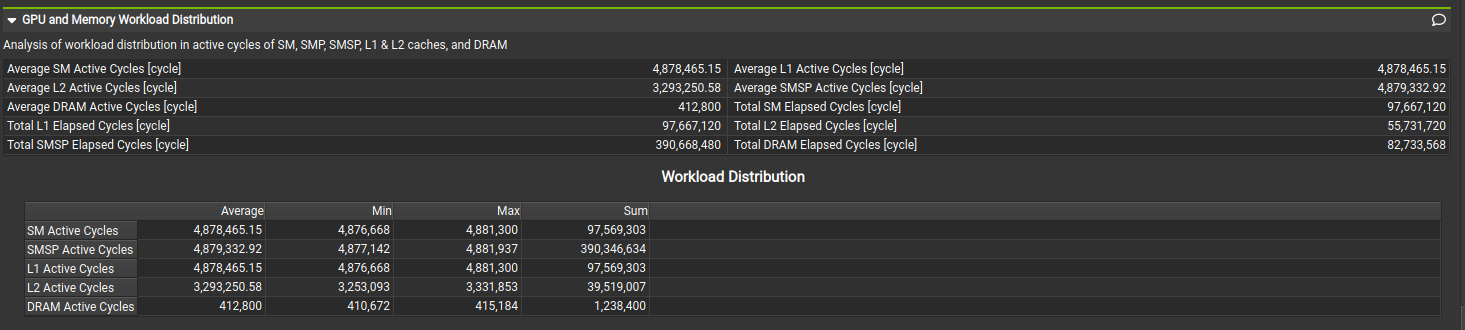
\includegraphics[width=0.95\linewidth]{figures/WorkloadDistribution.png}
    \caption{GPU and Memory Workload Distribution across Active Cycles}
    \label{fig:workload-distribution}
\end{figure}

\begin{figure}[H]
    \centering
    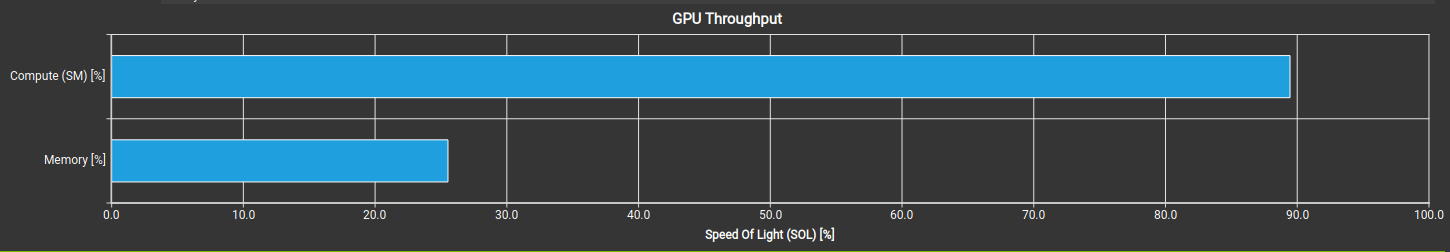
\includegraphics[width=0.9\linewidth]{figures/GPU_Throughput.png}
    \caption{Compute vs Memory Throughput as Percentage of Speed-of-Light}
    \label{fig:gpu-throughput}
\end{figure}

\textbf{Warp Behavior and Execution Bottlenecks.}

Figure~\ref{fig:warp-states} presents the breakdown of warp stalls. The most dominant stall reason was \textit{Tex Throttle}, followed by \textit{Short Scoreboard}, both indicative of memory-related latency.  
Figure~\ref{fig:pipe-utilization} further shows that the FP64 pipeline is over-utilized (89.5\% active cycles), potentially introducing bottlenecks.

\begin{figure}[H]
    \centering
    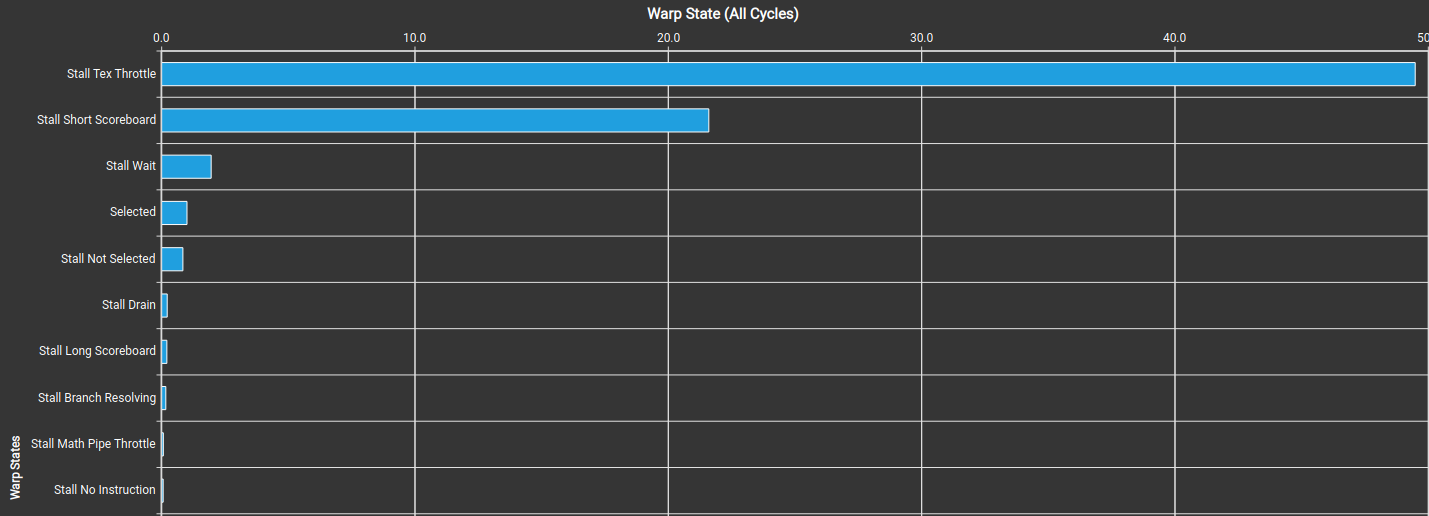
\includegraphics[width=0.95\linewidth]{figures/WarpState.png}
    \caption{Warp State Distribution during Kernel Execution}
    \label{fig:warp-states}
\end{figure}

\begin{figure}[H]
    \centering
    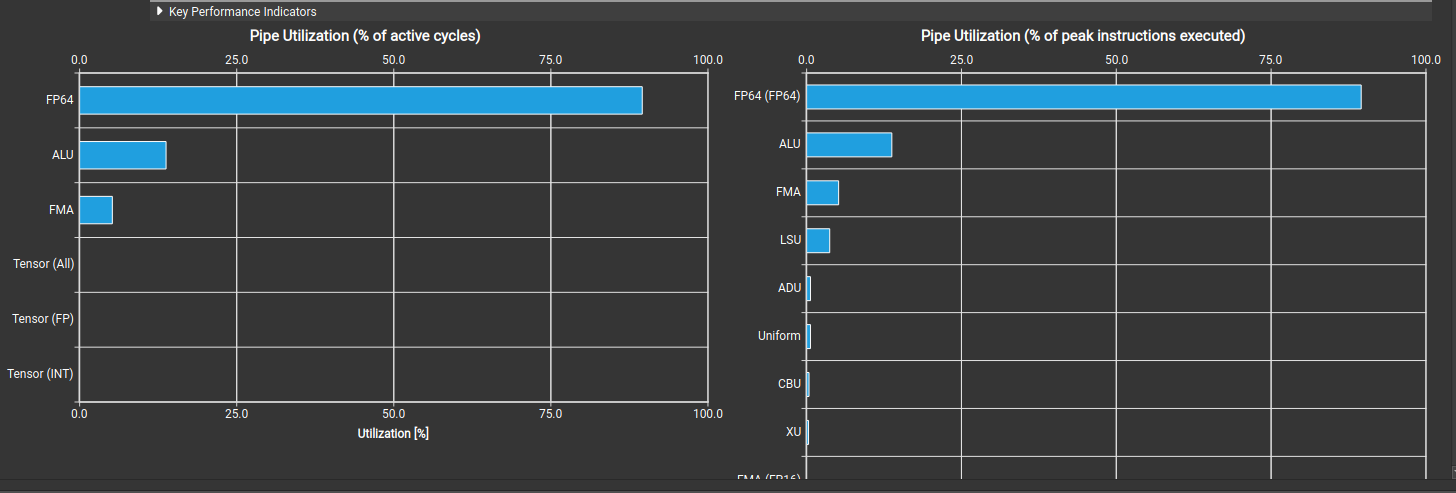
\includegraphics[width=0.95\linewidth]{figures/PipeUtilization.png}
    \caption{Pipe Utilization: FP64 Dominance and ALU/FMA Usage}
    \label{fig:pipe-utilization}
\end{figure}

\textbf{Memory Access and Cache Efficiency.}

Memory flow visualization in Figure~\ref{fig:memory-chart} shows strong L1/L2 cache performance with hit rates of 96\% and 98\% respectively.  
Figure~\ref{fig:l2-excess} shows that 94\% of L2 requests are uncoalesced, indicating room for improving memory access patterns via coalescing.

\begin{figure}[H]
    \centering
    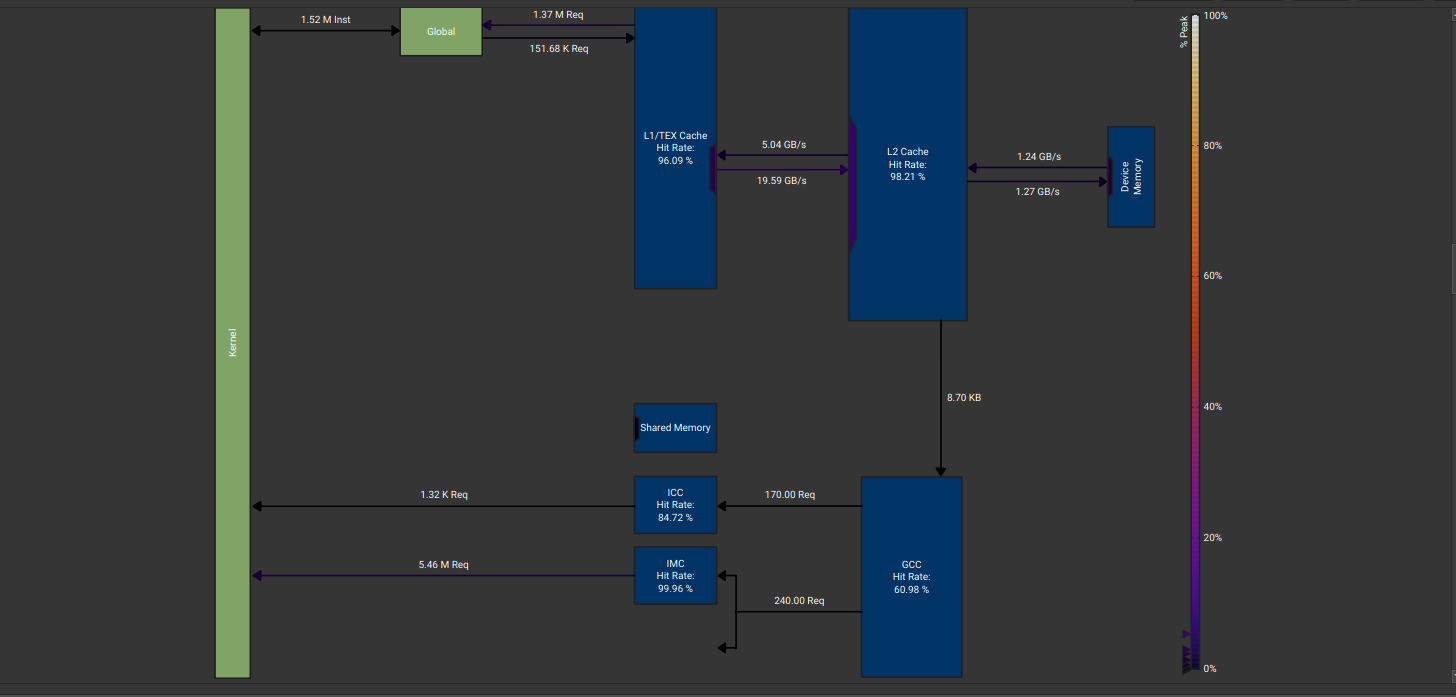
\includegraphics[width=0.9\linewidth]{figures/MemoryChart.png}
    \caption{Memory Access Pattern and Cache Hit Rates}
    \label{fig:memory-chart}
\end{figure}

\begin{figure}[H]
    \centering
    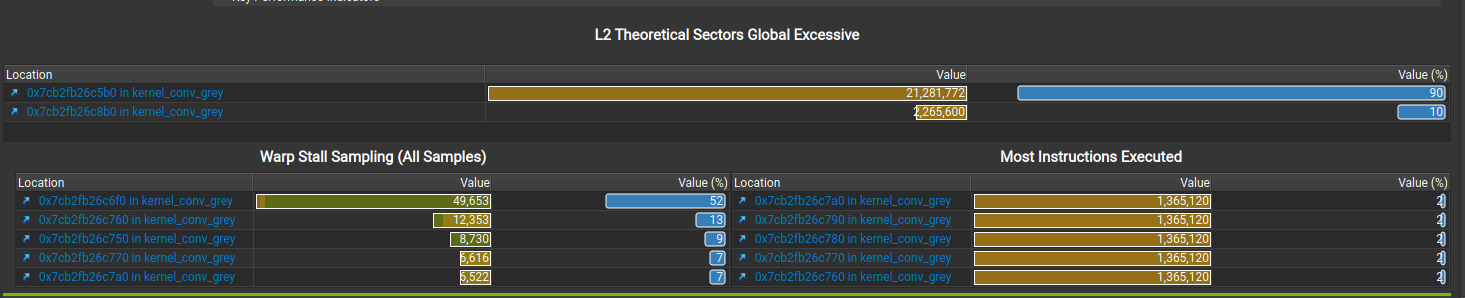
\includegraphics[width=0.9\linewidth]{figures/L2.png}
    \caption{L2 Cache: Global Access Sector Overuse and Warp Stalls}
    \label{fig:l2-excess}
\end{figure}

\textbf{Occupancy and Shared Memory Optimization.}

Nsight’s occupancy graphs (Figures~\ref{fig:occupancy-shared} and \ref{fig:occupancy-block}) show that using fewer registers and shared memory per block improves occupancy. The configuration around 256 threads per block with modest shared memory usage achieves optimal utilization.

\begin{figure}[H]
    \centering
    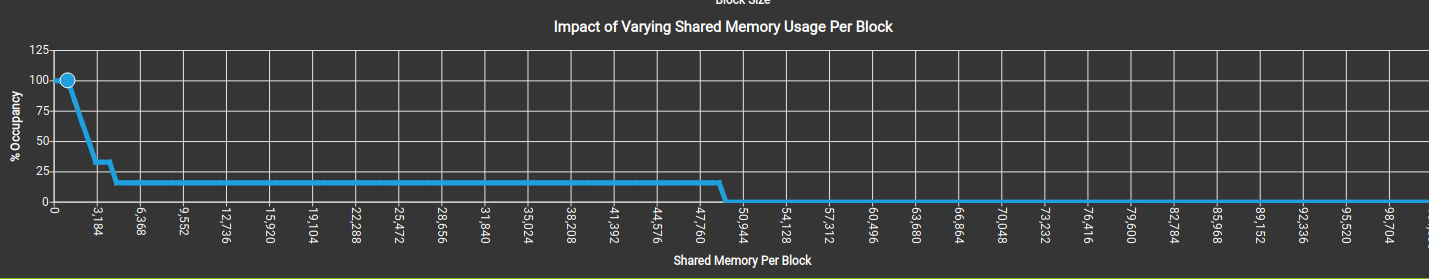
\includegraphics[width=0.9\linewidth]{figures/ImpactOfVarying_2.png}
    \caption{Occupancy vs Shared Memory Usage per Block}
    \label{fig:occupancy-shared}
\end{figure}

\begin{figure}[H]
    \centering
    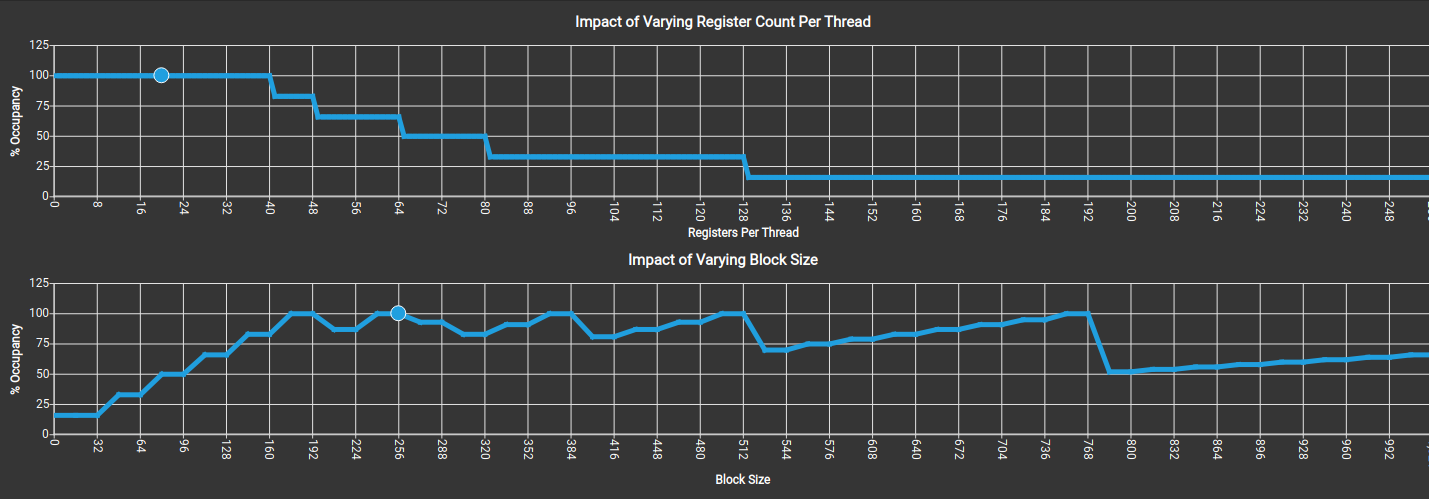
\includegraphics[width=0.9\linewidth]{figures/ImpactOfVarying.png}
    \caption{Occupancy vs Block Size and Register Usage}
    \label{fig:occupancy-block}
\end{figure}

\textbf{Performance Summary.}

The CUDA kernel demonstrated a speedup of over 11$\times$ compared to the sequential CPU implementation:

\[
\text{Speedup} = \frac{3100\text{ ms}}{265\text{ ms}} \approx 11.7\times
\]

\begin{table}[H]
    \centering
    \caption{Performance Comparison: CPU vs CUDA}
    \label{tab:speedup-table}
    \begin{tabular}{@{}lccc@{}}
        \toprule
        \textbf{Configuration} & \textbf{CPU Time (ms)} & \textbf{CUDA Time (ms)} & \textbf{Speedup} \\
        \midrule
        1920$\times$2520 Image & 3100 & 265 & 11.7$\times$ \\
        \bottomrule
    \end{tabular}
\end{table}

Overall, CUDA and Nsight Compute provided rich diagnostics, and the profiling insights suggest future directions for optimizing memory access patterns, reducing warp stalls, and increasing scheduler issue efficiency.




\subsection{\textbf{MPI}}

Benchmark workloads are chosen based on key criteria: representativeness, scalability, memory/computation balance, reproducibility, and their suitability for multi-core evaluation. The goal is to probe both compute-bound and memory-bound behaviors across a range of image sizes and convolution configurations.

\subsubsection{\textbf{Synthetic 2D Convolutions}}

To study the core computational kernel, we implement fixed-size 2D convolutions with square kernels over synthetic grayscale images \cite{Tousimojarad2017}.


\subsubsection{\textbf{Separable Filters}}

To evaluate the effects of cache reuse and two-pass access patterns, we implement separable convolutions.



\subsubsection{\textbf{End-to-End Image Processing Pipelines}}

To simulate realistic usage scenarios, we implement a three-stage filter pipeline.



\subsection{\textbf{OpenMp+MPI}}

To ensure accurate and reproducible performance results, our measurement methodology adheres to best practices drawn from recent literature on high-performance convolution and parallel computing \cite{Gawrych2023,  Rajput2013,  Yoon2012}.

\vspace{0.5em}
\textbf{1) Controlled Experimental Environment:} All benchmarks are run on a dedicated machine with minimal background activity. Turbo boost and dynamic frequency scaling are left enabled to reflect realistic performance, but measurements are conducted under stable thermal conditions.

\vspace{0.5em}
\textbf{2) Baseline Definition:} The sequential reference implementation is compiled with identical optimization flags as its parallel counterparts (\texttt{-O3}), and evaluated using the same input datasets. This ensures that any measured speedup reflects true parallel efficiency and not variation in compilation or execution environment.

\vspace{0.5em}
\textbf{3) Repeatability and Statistical Significance:} Each experiment is run 10 times after 3 warm-up iterations. The reported execution time is the arithmetic mean of the valid runs. We also calculate and report the standard deviation to capture runtime variability.

\vspace{0.5em}
\textbf{4) Timer Accuracy:} Wall-clock execution time is measured, which ensures consistency across operating system and hardware configurations. Timing includes only the kernel execution, excluding I/O and setup phases, unless otherwise noted.

\vspace{0.5em}
\textbf{5) Scaling Experiments:} 
We conduct both strong and weak scaling evaluations. For strong scaling, problem size remains fixed while thread count increases from 1 to 16. For weak scaling, the workload size grows proportionally with thread count to assess parallel overhead and memory behavior. Results will be interpreted in light of Amdahl’s Law, which characterizes the theoretical limits of strong scaling \cite{hager2021hpc}, and Gustafson’s Law, which describes expected performance under weak scaling \cite{Gustafson1988}.


\vspace{0.5em}
\textbf{6) Profiling and Hardware Analysis:} Low-level profiling is conducted using \texttt{perf}. We collect metrics such as cycles, instructions, cache misses, branch mispredictions, and memory bandwidth utilization. These metrics help correlate runtime behavior with architectural bottlenecks and assess the effectiveness.


\subsection{\textbf{Performance Metrics and Plots}}

To accurately convey both quantitative performance gains and underlying computational behavior, our evaluation will employ a selected set of performance metrics and visualizations. These choices follow established best practices from prior research in high-performance convolution and parallel computing \cite{Wang2023,  hager2021hpc, Rajput2013, Yoon2012}.

\vspace{0.5em}
\textbf{1) Speedup and Efficiency:} 
We will compute speedup as:
\begin{equation}
    S(p) = \frac{T(1)}{T(p)}
\end{equation}
and parallel efficiency as:
\begin{equation}
    E(p) = \frac{S(p)}{p}
\end{equation}
where \(T(1)\) is the execution time of the sequential version and \(T(p)\) is the time with \(p\) threads. These metrics will be plotted against thread counts to evaluate scalability and identify diminishing returns due to overheads or contention \cite{Rajput2013}.

\vspace{0.5em}
\textbf{2) Throughput and Kernel Performance:} 
We will report throughput in GFLOPS/s, defined by the theoretical number of floating-point operations in a convolution kernel divided by its execution time. This enables comparison with architectural peaks and identification of underutilization.

\textbf{4) Strong and Weak Scaling Curves:} 
We will generate strong scaling plots (fixed input size) and weak scaling plots (input size grows with thread count) to evaluate the scalability of our implementation. These plots will reveal how overheads such as synchronization and memory bandwidth contention grow with scale; their behavior will be interpreted in light of Amdahl’s Law and Gustafson’s Law as described in Section~3.3 \cite{hager2021hpc, Gustafson1988}.

\vspace{0.5em}
\textbf{5) Hardware Counter Visualizations:} 
Using \texttt{perf}, we will collect metrics such as cycles, instructions retired, L1/L2/L3 cache miss rates, and memory bandwidth. These will be plotted as bar charts or line graphs to explain bottlenecks and guide future optimization, as demonstrated in \cite{Yoon2012}.

\vspace{0.5em}
\textbf{6) Statistical Rigor:} 
All plots will be annotated with error bars reflecting the standard deviation over 10 runs. This practice enhances the interpretability of results and supports reproducibility by conveying variability in runtime behavior \cite{Yoon2012}.

Our chosen metrics and visualizations aim to support a rigorous, transparent, and insightful analysis of parallel performance across all stages of implementation and testing.





% ====================================================================
% --- END OF MAIN PROPOSAL CONTENT ---
% ====================================================================


\section*{Acknowledgment} 
% Add acknowledgments
We thank Dr. Islam Tharwat Abdel Halim and Eng. Hassan Ahmed for their guidance.


% --- Bibliography Setup (Keep these lines) ---
\bibliographystyle{IEEEtran} 
\bibliography{references} % file is references.bib

\end{document}
% --- END OF FILE proposal.tex ---